\documentclass[a4paper,10pt,titlepage]{paper}

\usepackage[utf8]{inputenc}
\usepackage[T1]{fontenc}
\usepackage[english]{babel}
\usepackage{amssymb}
\usepackage{mathtools}
\usepackage{bchart}
\usepackage{color}
\usepackage{xcolor}
\usepackage{listings}
\usepackage[style=ieee, defernumbers=true, backend=bibtex]{biblatex}

\bibliography{referencer}

\usepackage{float}
\usepackage{hyperref}
\hypersetup{%
    pdfborder = {0 0 0}
}

\parindent0em

\lstset{%
mathescape,
frame=single,
numbers=left,
numberstyle=\footnotesize,
tabsize=4,
keepspaces=true,
columns=fullflexible,
basicstyle=\normalsize,
inputencoding=utf8,
extendedchars=true,
}
\renewcommand{\lstlistingname}{Algorithm}% Listing -> Algorithm
\usepackage{fancyhdr}
\usepackage{lastpage}


\fancyhf{} % resetting the header and footer
\pagestyle{fancy} % using fancyhdr to make custom header and footer 
\lhead{Henrik Schulz} % left header
\lfoot{} % left footer
\chead{}
\rhead{31. December 2017} % right header
\rfoot{Page \thepage\ of \pageref{LastPage}} % right footer
\renewcommand{\headrulewidth}{0.0pt} % removing the header separtions line

\title{Computational Synthesis Planning Using Big Data}
\author{Computational Syntese planlægning ved hjælp af big data\\ \\Master Thesis 2018\\Henrik Schulz}
\date{31/12/2017}

\begin{document}
\begin{titlepage}

\newcommand{\HRule}{\rule{\linewidth}{0.5mm}} % Defines a new command for the horizontal lines, change thickness here

\center % Center everything on the page

\textsc{\LARGE University of Southern Denmark\\\vspace{0.2cm}Department of Mathematics \\ \vspace{0.2 cm} and Computer Science}\\[1.5cm] % Name of your university/college
\textsc{\large Master Thesis -- 31/12-2017}\\[0.5cm] % Major heading such as course name

\HRule \\[0.4cm]
{\huge \bfseries Computational Synthesis Planning Using Big Data}\\[0.4cm] 
{Computational Syntese planlægning ved hjælp af big data}
\HRule \\[1.5cm]

\begin{minipage}{0.3\textwidth}
\begin{flushleft} \large
\emph{Author:}\\
Henrik Schulz\\

\end{flushleft}
\end{minipage}
~
\begin{minipage}{0.4\textwidth}
\begin{flushright} \large
\emph{Supervisors:} \\
Daniel Merkle
\end{flushright}
\end{minipage}\\[4cm]

\includegraphics[scale=0.3]{Billeder/logo.png}
\vfill % Fill the rest of the page with whitespace

\end{titlepage}

\vfill
\section*{Abstract}

\section*{Resumé}
\newpage

\tableofcontents
\newpage


\section{Acknowledgements}

\section{Introduction}
kkk \cite{Grzybowski}\\
\subsection{Overview}
Hvad indeholder hver sektion??

\section{Preliminaries}

This section contains definitions that will be used throughout this paper. It is assumed that the reader have a basic understanding of graph theory. \\

\textbf{Hypergraphs}\\
A directed hypergraph $h$ is a set of $V$ of vertices and a set $E$ of hyperedges, where each hyperedge $e=(T(e),H(e))$ is an ordered pair of non-empty multi-sets of vertices. The set $T(e)$ is denoted as the tail of the hyperedge and $H(e)$ is the head. If $|H(e)|=1$ then the hyperedge is denoted as a B-hyperedge. If all edges in the hypergraph is B-hyperedges, then the graph is denoted a B-hypergraph. This paper will only consider hypergraphs that are B-hypergraphs. A hypergraph $H' = (V',E')$ is a subhypergraph of $H=(V,E)$ if $V' \subset V$ and $E'\subset E$.\cite{Fagerberg}

\begin{figure}[H]
\centering
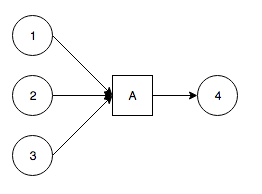
\includegraphics[scale=0.5]{Billeder/HyperEdge.png}
\caption{Example of hyperedge $A$. $T(A) = \{1,2,3\}$, $H(A) = \{4\}$}
\end{figure}

\textbf{Hyperpaths}\\
A path $P_{st}$ from $s$ to $t$ in a B-hypergraph is a sequence $P_{st}=\langle e_1, e_2, e_3, ... , e_q \rangle$ of B-hyperedges such that $s\in T(e_1)$ and $t=H(e_q)$ and $H(e_i) \in T(e_{i+1})$ for $i=1..q-1$. Its length $|P_{st}|$ is the number $q$ of hyperedges. If $t \in T(e_1)$, then $P_{st}$ is a cycle. A hypergraph is acyclic if it does not contain any cycles. \cite{Fagerberg}

\section{Finding The K-Best Synthetic Plans}
kkk \cite{Carsten}\\
kkkk \cite{Fagerberg}\\
\subsection{Yen's Algorithm}
Yen's algorithm is an algorithm that computes the K-shortest paths for a graph with non-negative edges. It was publish in 1971 and uses any shortest path algorithm to find the best path and then proceeds to find the $K-1$ deviation of the best path. \cite{Yen}

It starts out by finding the best path using a shortest path algorithm. Once the best path have been found it uses the path to find all the potential next best paths by fixing and removing edges in the graph. \\
By using the same first vertex as the original path but removing the first edge, it forces the shortest path algorithm to take another route through the graph and thereby creating a potential second best path. This is added to the list of potential paths and the algorithm can continue to derive other paths from the best path. By fixing the first edge in the previous best plan, Yen's algorithm forces the shortest path algorithm to take the first edge which it now shares with the best path. However, now the algorithm have removed the second edge from the original path and once again forces the shortest path algorithm to find alternative routes. This process is then repeated until we reach the next to last vertex in the best path.\\
By sorting the list of potential paths, it has the second best path at the start of the list and it can add it to the final list of best path. The algorithm then repeats on the second best path to find the third best path. This is done until all K-best path have been found.

\subsection{Yen's Algorithm On Hypergraphs}
We use the principles from Yen's algorithm to make our own algorithm that will work on hypergraphs. To handle the problem of generating all derived paths from our best path in our hypergraph, we use a method called BackwardsBranching. \cite{Fagerberg} \cite{Nielsen} \cite{Carsten}
\begin{lstlisting} [emph={if,for, endif, endfor, function, endfunction, do}, emphstyle = \bfseries,caption = Backwards Branching for B-Hypergraph]
function Back-Branch(H,$\pi$)
	B=$\emptyset$
	for i = 1 to q do 
		Let H$^i$ be a new hypergraph
		H$^i$.V = H.V
		// Remove hyperarc from H
		H$^i$.E = H.E $\setminus \{\pi.p(v_i)\}$
		// Fix Back tree
		for j = i+1 to q do
			H$^i$.BS(vj) = \{$\pi.p(v_j)$\}
		B = B $\cup$ \{H$^i$\}
	return B
\end{lstlisting}
However, this algorithm have a problem when working on a larger hypergraph. It demands that each time we make alterations on the hypergraph we have to make a copy, $H^i$, of the graph, $H$, with the exception of the hyperedges that is removed when fixing the back tree and removing $\pi.p(v_i)$.\\
This could easily work for smaller graphs, but if we use this on the hypergraph that we generate from the beilstein database, we would have to copy a graph of multiple GigaBytes. \\
To handle this problem I came up with the idea of creating an overlay for the graph instead of copying it. The overlay would work as an transparent on top of the original graph, stating which edges still were accessible. This is done by creating a \textit{vector<bool>} which has a length of $R$, where $R$ is the number of reactions. Normally a reaction would contain at least 24 bytes of data:
\begin{itemize}
\item
2x ints of 4 bytes each
\item
1x double of 8 bytes
\item
1x \textit{vector<int>} head of length one of at least 4 bytes
\item
1x \textit{vector<int>} tail of length $N$ (number of educts) of at least 4 bytes
\end{itemize}
This can be reduced dramaticly by using the \textit{vector<bool>}, since c++ only uses 1 bit per boolean in the vector instead of the regular 1 byte per boolean.\cite{VectorBool} This means if working on a hypergraph with 40 million reactions, we would be able to create an overlay using 5 MB of space per alternated graph, instead of copying a hypergraph were the reactions alone uses at least 960 MB per copy. \\
As the figure below shows, we never change or remove anything on the hypergraph. We simply create the following overlay:
\begin{table}[H]
\centering
\begin{tabular}{c|c|c|c|c}
Reaction & A & B & C & D \\\hline
Usable & true & true & true & false \\\hline
Bit Representation & 1 & 1 & 1 & 0
\end{tabular}
\end{table} 
And then when trying to use an edge, we simply ask: "Does overlay at reaction A exist?". If yes, you can use it. If no, the edge have been "removed", and therefore cannot be used.
\begin{figure}[H]
\centering
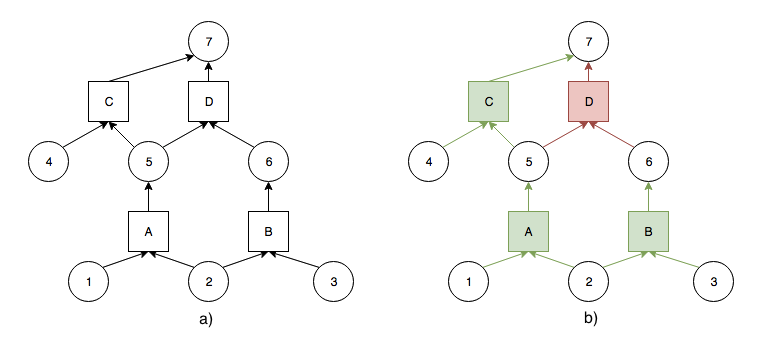
\includegraphics[scale=0.5]{Billeder/OverlayIllustration}
\caption{a) The original hypergraph. b) The original hypergraph, but using the overlay. If the reaction is green it is still usable. If red then it have been "removed" from the hypergraph.}
\end{figure}

This of course means that the algorithm for back-branch have to be changed accordingly. Instead of the hypergraph as input we now give it an overlay. This overlay is changed so it fits with the new layout of the graph. Instead of deleting hyperedges in the copy, we now simply changes the boolean at the index of the hyperedge.id. True if we should add the hyperedge and false when we want to "remove" a hyperedge.

\begin{lstlisting} [emph={if,for, endif, endfor, function, endfunction, do}, emphstyle = \bfseries,caption = Backwards Branching for B-Hypergraph using overlay]
function BackwardsBranching($\pi$, Overlay) 						
	List B = $\emptyset$
	// q = Path length
	for i = 1 to q do			
		//remove i'th hyperedge from Path in overlay					
		Set Overlay[$\pi$[i]] to false		
		//fix the backtree				
		for j = i downto 1	do							
			vertex C <- $\pi$[j].head
			for each hyperedge into C
				Set Overlay[reaction.id] to false
			Set Overlay[$\pi$[j]] to true
		endfor
		B = B $\cup $ {$Overlay$}
	endfor
	return B
endfunction
\end{lstlisting}

\begin{lstlisting} [emph={if,for, endif, endfor, function, endfunction, do}, emphstyle = \bfseries,caption = K-Shortest Paths Algorithm in B-Hypergraph]
function YenHyp(s, t, K) 
	L = new heap with elements (overlay, maxYield)
	A = List of shortest paths
	//(Graph is default overlay (all true))
	$\pi$ = shortestPath(Graph, s,t) 				
	Insert (Graph, $\pi$) into L
	for k = 1 to K do
		if L = $\emptyset$
			Break
		endif
		(Overlay$'$, $\pi'$) = L.pop
		for all Overlay$^i$ in BackwardBranching((Overlay$'$,$\pi'$)) do
			$\pi^i$ = shortestPath(Overlay$^i$, s, t)
			if $\pi^i$ is complete
				Insert( $H^i$, $\pi^i$) into L
			endif
		endfor
	endfor
	return A
endfunction
\end{lstlisting}

\section{Shortest Path}
\subsection{Dynamic Approach}
kkk \cite{Carsten}\\
kkkk \cite{Fagerberg}\\

\subsubsection{Approach}
\subsubsection{Testing}
\subsubsection{Problems}

\subsection{Nielsens Algorithm}
k \cite{Nielsen}
\subsubsection{Approach}
\subsubsection{Testing}
\subsubsection{Optimizing}

\section{Work With Beilstein Data}
\subsection{The Graph}
\subsection{Testing}
\subsubsection{Strychnine}
\subsubsection{Compound 2} 
\subsubsection{Compound 3}
kkkk \cite{SynthesisPlans}\\

\section{Konklusion}

\newpage

\printbibliography[type=book, title={Books}]
\printbibliography[type=article, title={Articles}]
\printbibliography[nottype=book, nottype=article, title={Other}]

\newpage
\section{Appendiks}

\end{document}